\documentclass[11pt]{article}

% Official ACL layout, with author names visible for the course submission.
\usepackage[final]{acl}
\usepackage{times}
\usepackage{latexsym}
\usepackage[T1]{fontenc}
\usepackage[utf8]{inputenc}
\usepackage{microtype}
\usepackage{inconsolata}
\usepackage{amsmath,amssymb}
\usepackage{graphicx}
\usepackage{booktabs}
\usepackage{array}
\usepackage{dsfont}
\usepackage{xcolor}
\usepackage{listings}
\lstset{basicstyle=\ttfamily\scriptsize, breaklines=true, breakindent=0pt, columns=fullflexible,
  keepspaces=true, frame=single, framerule=0.4pt, rulecolor=\color{gray}, aboveskip=2pt, belowskip=6pt}
% \FloatBarrier before each appendix section keeps its figures and tables inside it.
\usepackage{placeins}

% Keep citations and references black while preserving clickable links.
\hypersetup{hidelinks}
% Keep at least two paragraph lines together at column/page boundaries.
\clubpenalty=10000
\widowpenalty=10000
\displaywidowpenalty=10000

% Course limit: 5 pages of main content, excluding references.
% Keep the ACL margins, fonts, and body line spacing unchanged.
\title{How Invariant is Code Generation to Graph Serialization?\\
  Measuring and Localizing the Fragility}

\author{
  \normalfont
  \begin{tabular}{@{}c@{\quad}c@{\quad}c@{\quad}c@{}}
    \textbf{Ram Kedem} & \textbf{Yehonatan Barel} & \textbf{Ido Azoulay} & \textbf{Dolev Abudi} \\
    206844144 & 208646422 & 212710958 & 323096099
  \end{tabular} \\[12pt]
  \normalfont\normalsize Code and data: \url{https://github.com/dolev98/graph_serialization_invariance}
}

\begin{document}
% Keep natural paragraph spacing instead of stretching gaps to fill columns.
\raggedbottom
\maketitle

\begin{abstract}

Language models often answer graph questions better by writing code than by answering directly. However, the answer can depend on how the graph is serialized, and a correct answer for one serialization does not guarantee a correct answer for another. We ask: \emph{does solving a graph problem using code generation return the same answer under equivalent serializations of the same graph, and if not, at which step does the fragility enter?} Across four models and two datasets, changing one aspect of the serialization at a time, we find that code generation is far more robust to the serialization, changing its answer two to five times less often than direct answering, a gap that grows with graph size, yet no condition in which the model reads the graph is fully invariant. The fragility enters mostly in the program the model writes, not in its copy of the graph. We also find that keeping the graph out of the prompt nearly removes the sensitivity at no cost in accuracy.
\end{abstract}

\section{Introduction}

Large language models typically receive graphs as serialized text. The choice of serialization affects both accuracy \citep{fatemi} and permutation invariance: renaming nodes or reordering edges leaves the graph and the question unchanged, yet can change the answer \citep{ge,herbst}. Code generation has proved one of the strongest ways to answer graph questions \citep{cai,finkelshtein}, but higher accuracy does not necessarily mean invariance across serializations \citep{herbst}.

 We send each graph question to the model in three ways. In direct answering (M1), the model reads the serialized graph and replies with the answer. In code from text (M2), it reads the same graph and replies with a Python program that copies the graph and computes the answer when we run it. In Graph-as-Code (M3), it writes the program from the question alone, and we pass the graph to the program as data when we run it. Comparing M1 with M2 shows whether code generation comes closer to serialization invariance: returning the same answer for every equivalent serialization of the same graph. The M2 programs show where the remaining violations enter, in the model's copy of the graph or in the program it writes. M3 tests whether keeping the graph out of the prompt restores invariance without losing accuracy. 

Our contributions are as follows. (i) A per-instance, single-factor invariance measurement of \emph{executed} code over four models and two datasets. (ii) Evidence that when the answer changes, the cause is rarely a wrong copy of the graph but the program the model writes. (iii) Evidence that keeping the graph out of the prompt nearly removes the sensitivity at no cost in accuracy, provided the prompt states the graph type.

\section{Related Work}

\textbf{Graph reasoning from text.} NLGraph \citep{wang} and GraphQA \citep{fatemi} showed that LLMs solve small graph problems posed in text, but unreliably: on GraphQA the best and worst encodings of the same graphs differ by 4.8 to 61.8 points for PaLM 62B. Erdős \citep{guo} extends evaluation to 50 tasks.

\textbf{Serialization invariance.} The order of a graph's description alone shifts accuracy \citep{ge}, and \citet{herbst}, varying node labels, computational structure and syntax one at a time, find that each factor changes outputs. Their models answer directly, reading NetworkX code as text rather than running it, and their per-example measure covers numeric answers only. We measure per-instance agreement on executed code, for every answer type.

\textbf{Computing with code.} Program-aided reasoning hands the computation to an interpreter \citep{gao}. CodeGraph \citep{cai} has GPT-3.5 write Python for GraphQA tasks, and across six encodings its best-worst accuracy gap is smaller than under chain-of-thought on every task. \citet{finkelshtein} find code generation the strongest interaction mode for node classification on text-rich graphs. Neither tests invariance: \citet{finkelshtein} use a single serialization, and CodeGraph compares aggregate accuracy over encodings that change several factors at once. Its one-shot example also supplies the solving function, so its model need only copy the graph, not write the solving step, where we find the failures.

\section{Methodology}

Each \emph{instance} is a graph, a question about it and the correct answer. We write each graph in several equivalent serializations, pose each one in three interaction modes, and check whether the answers stay the same and are correct.

\subsection{Data}

We use two benchmarks, one with basic graph questions and one with harder algorithmic tasks.

\textbf{GraphQA:} This benchmark \citep{fatemi} asks basic questions, such as edge existence, node degree and cycle detection, about small random graphs (5-20 nodes) built by seven graph generators. We follow its recipe to generate 100 graphs and ask one question of each of seven question types on every graph, giving 700 instances.

\textbf{Erdős:} This published suite \citep{guo} covers 50 harder algorithmic tasks and is the one \citet{herbst} used. We take 12 of its tasks, such as shortest path, triangle counting and bridges, with 100 test graphs each (4-34 nodes).

\subsection{Interaction Modes}\label{sec:modes}

\textbf{Direct answering (M1):} The model reads the serialized graph and the question and answers directly. This is the known fragile baseline \citep{herbst}.

\textbf{Code from text (M2):} The model gets the same input and writes a Python program that we execute. The program must start by writing out the graph as a list of nodes and a list of edges, so we see exactly what the model copied.

\textbf{Graph-as-Code (M3):} In this mode, adapted from \citet{finkelshtein}, the model sees only the task and the question and writes code over a list of nodes and a list of edges that it never sees. We fill these lists with the serialized graph at execution.

Both code modes run in two library arms: native, limited to the Python standard library so that the model writes the algorithm itself, and NetworkX allowed. Figure~\ref{fig:A1} in Appendix~\ref{app:prompts} shows the prompts of the three modes for one instance.

\subsection{Serialization Factors}\label{sec:factors}

The baseline serialization is the dataset's own edge list. Every other serialization changes exactly one of four factors, so that a change in the answer can be attributed to that factor. \textbf{Relabeling} applies a random permutation of the node labels to the graph and to the question and maps node-valued answers back. \textbf{Order} lists the edges in three orderings: sorted by the first endpoint, by the second, or shuffled. \textbf{Structure} adds two serializations: an adjacency list, and, for undirected graphs, an edge list in which each edge is written twice, as (u, v) and (v, u). \textbf{Syntax} writes the same edge list as plain text, JSON or NetworkX code (Erdős: JSON and NetworkX code only).

\section{Experimental Setup}

\subsection{Models}

We test four models of different sizes: Qwen3-8B (Alibaba, 8B parameters), Gemma 4 31B (Google, 31B), DeepSeek-V4-Flash (284B, of which 13B are active for each token) and DeepSeek-V3.1 (671B, 37B active).

\textbf{Inference:} All four models run through the same API gateway with the same settings: temperature 0, at most 4,096 output tokens, and reasoning turned off, so that direct answering stays a direct answer rather than a hidden chain of thought. Generated programs run in a separate process with a time limit.

\textbf{Scale:} Each model answers every serialization of every instance in all five conditions (Section~\ref{sec:modes}): 44,625 answers per model on GraphQA and 71,230 on Erdős.

\subsection[Metrics]{Metrics}\label{sec:metrics}

\textbf{Terms:} A \emph{factor} is the kind of change: relabeling, edge order, structure or syntax (Section~\ref{sec:factors}). A \emph{serialization} is one concrete text of a graph. A \emph{tuple} collects the answers one model gives, in one interaction mode, to the serializations of one instance under one factor (Figure~\ref{fig:1}). Under relabeling, for example, a tuple holds four answers: to the baseline labeling and to three random relabelings. Table~\ref{tab:D1} in Appendix~\ref{app:tuples} gives the tuple sizes.

\textbf{Correctness:} An answer is correct when it equals the true answer. When a question has several correct answers, for example two equally short paths, any of them is correct. Real-valued answers are compared with a small tolerance. A crash, a timeout or an unreadable reply counts as wrong.

\textbf{Performance:} Accuracy is the share of all answers that are correct. Robust accuracy is the share of tuples in which every answer is correct.

\textbf{Invariance:} A tuple \emph{flips} when at least one of its answers differs from the others. When a question has several correct answers, they count as the same answer, and a missing answer counts as an answer of its own. The flip rate is the share of tuples that flip. Crossing the flips with correctness divides the tuples into six buckets (Table~\ref{tab:1}): (1) the same correct answer on every serialization, (2) the same wrong answer, (3) different answers that are all correct, (4) a flip in which every serialization is answered, (5) a flip with a crash, and (6) no answer on any serialization.

\textbf{Weighted flips:} The flip rate treats every flip alike, whether one answer deviates or all of them differ. We therefore define two measures on a tuple with answers $a_1, \ldots, a_n$ and true answer $y$. $D$ is the fraction of answer pairs that differ, and $S$ is the range of the answers relative to the true answer:
\begin{gather*}
D = \frac{1}{\binom{n}{2}} \sum_{1 \le i < j \le n} \mathds{1}\left[a_i \neq a_j\right], \\
S = \frac{\max_{i} a_i - \min_{i} a_i}{|y|}
\end{gather*}

$D$ is 0 when all answers agree and 1 when all differ: (1, 2, 2, 2) has $D = 0.5$ and (1, 2, 3, 4) has $D = 1$. $S$ applies to numeric answers, and $S = 1$ means the answers span the whole true value, as when a count doubles. The mean of $D$ over flipped tuples is the \emph{severity} of the flips.

\textbf{Localization:} We trace M2 failures to one of three steps: the copy of the graph (the program declares a wrong graph), a crash (it gives no answer) or the program's solving step (otherwise). Each wrong answer is assigned the first of these steps that failed, and each flipped tuple the step at which its serializations diverge.

\textbf{Statistics:} Every rate is computed per dataset, mode and factor, with the four models weighted equally. Brackets are 95\% confidence intervals with errors clustered by graph, and whiskers are 95\% bootstrap intervals over graphs.

\section{Results and Discussion}

\subsection{Does executed code keep its answer, and more often than direct answering?}\label{sec:rq1}

Executed code flips far less often than direct answering, but is still not invariant (Figure~\ref{fig:2}). Under relabeling and edge order, direct answers (M1) flip on 11.9\% of GraphQA and 20.8\% of Erdős tuples. Code from text (M2) flips on 4.8\% and 3.5\% in plain Python and 6.8\% and 4.5\% with NetworkX. Code flips significantly less (McNemar's test) in 14 of 16 model $\times$ dataset $\times$ code library cells. Both exceptions are Gemma 4 31B on GraphQA, whose direct answers are already the most stable (3.0\%). In a logistic regression with model, task and factor held fixed, M2's plain-Python code has 0.47 [0.41, 0.54] times direct answering's odds of a flip on GraphQA and 0.20 [0.17, 0.22] on Erdős, and NetworkX code 0.52 [0.44, 0.61] and 0.31 [0.27, 0.36]. Figures~\ref{fig:B1} and~\ref{fig:B2} give each model.

\begin{figure}[t]
\centering
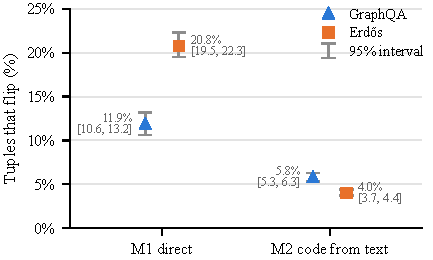
\includegraphics[width=0.85\columnwidth]{figures/fig2_flip_by_mode.pdf}
\caption[Flip rate under relabeling and edge order]{ Flip rate under relabeling and edge order, with M2 averaged over plain Python and NetworkX. Whiskers are 95\% bootstrap intervals over graphs.}
\label{fig:2}
\end{figure}

On Erdős, code's flips are also milder (Figure~\ref{fig:3}). Four in five plain-Python flips have a single serialization out of line ($D = 0.5$), against two in five for direct answering. Severity is 0.54 against 0.71, so weighting by $D$ widens the gap from 6$\times$ to 8$\times$.

The gap grows with the graph (Figure~\ref{fig:4}). From graphs with up to 10 edges to graphs with more than 40, direct answering's flip rate rises from 7.7\% to 23.1\% on GraphQA and from 6.1\% to 36.2\% on Erdős, while code stays between 1.5\% and 8.2\%. In a logistic regression with task and model held fixed, each doubling of the edge count multiplies direct answering's odds of a flip by 1.60 [1.46, 1.74] on GraphQA and 2.44 [2.19, 2.71] on Erdős, and plain-Python code's by 0.96 [0.86, 1.08] and 1.52 [1.34, 1.72].

\begin{figure}[t]
\centering
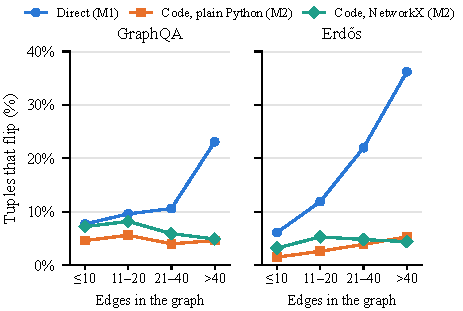
\includegraphics[width=\columnwidth]{figures/fig4_graph_size.pdf}
\caption{Share of tuples that flip under relabeling and edge order, by the number of edges, four models pooled.}
\label{fig:4}
\end{figure}

Although we use temperature 0, the same prompt asked again can get a different answer, so part of every flip rate is noise. Only Qwen3-8B's code clearly exceeds this repeat floor. Under the same flip rule, Qwen3-8B's code exceeds it in all 8 cells, by 4.0-11.0 points, while the other three models' code does so in only 3 of 24.

A stable answer is not always a correct one (Table~\ref{tab:1}, per model in Table~\ref{tab:B1}). On GraphQA, 8.1\% of plain-Python tuples give the same wrong answer on every serialization. Most of them come from one question, which nodes are not connected to a given node, where DeepSeek-V3.1 and DeepSeek-V4-Flash both list the nodes it cannot reach instead of those without a direct edge to it. Invariance cannot see these errors, so we report robust accuracy beside it (Table~\ref{tab:3}).

\begin{table}[t]
\centering
\small\setlength{\tabcolsep}{3.2pt}
\begin{tabular}{@{}lrrrrrr@{}}
\toprule
 & \multicolumn{3}{c}{GraphQA} & \multicolumn{3}{c}{Erd\H{o}s} \\
\cmidrule(lr){2-4} \cmidrule(l){5-7}
Bucket & Dir. & Py & NX & Dir. & Py & NX \\
\midrule
(1) Same, correct & 76.7 & 87.2 & 85.4 & 74.9 & 91.3 & 85.8 \\
(2) Same, wrong & 11.4 & 8.1 & 7.7 & 0.5 & 0.6 & 0.3 \\
(3) Different, all correct & 0.0 & 0.0 & 0.0 & 3.8 & 4.5 & 4.3 \\
(4) Flip, all answered & 11.5 & 4.7 & 5.5 & 17.6 & 2.7 & 0.9 \\
(5) Flip with a crash & 0.3 & 0.0 & 1.2 & 3.2 & 0.9 & 3.6 \\
(6) No answer on all & 0.0 & 0.0 & 0.1 & 0.0 & 0.0 & 5.0 \\
\bottomrule
\end{tabular}
\caption{Tuples by bucket under relabeling and edge order, \% of tuples, four models pooled. Buckets 4 and 5 are the flips. Dir. = M1. Py and NX = M2 in plain Python and with NetworkX.}
\label{tab:1}
\end{table}

\subsection{Which factor flips the answer?}\label{sec:factor-results}

Edge structure flips plain-Python answers the most, and NetworkX-code syntax flips NetworkX answers by crashing the programs. Relabeling and order permute the same text, and code barely reacts to them: 3.5-7.2\% of code tuples flip (Table~\ref{tab:2}, per model in Table~\ref{tab:B2}). In the same logistic regression, structure raises the odds of a flip relative to relabeling 2.18-fold [1.99, 2.39] on GraphQA and 1.68-fold [1.55, 1.83] on Erdős, and syntax 1.42-fold [1.29, 1.56] and 1.45-fold [1.35, 1.56].

\begin{table}[t]
\centering
\small\setlength{\tabcolsep}{3.2pt}
\begin{tabular}{@{}lrrrrrr@{}}
\toprule
 & \multicolumn{3}{c}{GraphQA} & \multicolumn{3}{c}{Erd\H{o}s} \\
\cmidrule(lr){2-4} \cmidrule(l){5-7}
Factor & Dir. & Py & NX & Dir. & Py & NX \\
\midrule
Relabeling & \textbf{12.6} & 5.6 & 7.2$^\dagger$ & \textbf{22.1} & 3.6 & 4.7 \\
Order & \textbf{11.1} & 4.0 & 6.3$^\dagger$ & \textbf{19.6} & 3.5 & 4.3 \\
Structure & \textbf{19.2} & \textbf{18.5}$^\dagger$ & 8.0 & \textbf{19.5} & \textbf{13.7} & \textbf{10.2} \\
Syntax & \textbf{14.9} & 4.8 & \textbf{13.6}$^\dagger$ & \textbf{18.9} & 3.8 & \textbf{16.6}$^\dagger$ \\
\bottomrule
\end{tabular}
\caption[Flip rate by factor]{ Flip rate by factor (\% of tuples, models pooled). Bold: 10\% or more. $^\dagger$: some model's code flips at least 1 point more than its direct answers. Dir. = M1. Py, NX = M2 in plain Python and NetworkX.}
\label{tab:2}
\end{table}

\textbf{Structure:} Listing each undirected edge in both directions makes plain-Python programs count it twice, and 18.5\% of GraphQA and 13.7\% of Erdős tuples flip. On GraphQA node degree, 176 of Qwen3-8B's 200 answers are exactly double the true degree. These flips are far off, not just different: their median spread $S$ is 1.0 on both datasets, and 93\% (GraphQA) and 49\% (Erdős) contain an exact doubling. A NetworkX \texttt{Graph} merges the duplicates, so NetworkX code flips less (8.0\% and 10.2\%). Accuracy follows: structure costs plain-Python code 9.8 points on GraphQA and 6.7 on Erdős, while relabeling and order cost code at most 0.7.

\textbf{Syntax:} When the graph arrives as NetworkX code, NetworkX programs crash on some serializations and not on others, and 13.6\% and 16.6\% of tuples flip. Qwen3-8B's programs leave out the import, and DeepSeek-V4-Flash's use a \texttt{G} they never define, both as if the prompt's code had already run. Without these two crashes, which cause 51\% (GraphQA) and 71\% (Erdős) of the flips, NetworkX code would flip on 6.6\% and 4.8\%, about as often as under relabeling and order. The syntax costs NetworkX code 6.2 points of accuracy on Erdős, while plain-Python code is unaffected (4.8\% and 3.8\% flip).

\subsection{Which failures accompany a flip?}\label{sec:localize}

Most flips start in the program the model writes, and few in its copy of the graph. The graph a program declares matches the input in 98.1-99.9\% of code answers. Among failed plain-Python answers, the solving step accounts for 97.8-99\% on GraphQA and 77-81\% on Erdős, while with NetworkX crashes account for 63-97\% of Erdős failures. A wrong copy is at most about 13\% of failures, and it does not reveal itself: 64\% (GraphQA) and 60\% (Erdős) of programs that declare a wrong graph still answer correctly.

Failures are not flips, though, so Figure~\ref{fig:5} attributes each flip itself to where its serializations diverge. On GraphQA, 95.5\% of plain-Python flips start in the program. On Erdős the program still leads (61.5\%, mostly Qwen3-8B's), but a crash starts 20.9\%, mostly DeepSeek-V4-Flash's, and a wrong copy 17.6\%: 35 of DeepSeek-V3.1's 40 flips come from a wrong copy of a long edge list.

The M3 control points the same way: under edge order, Graph-as-Code runs one fixed program on every ordering and flips on 0.0-0.1\% of tuples, against 3.5-6.3\% for M2. Since M3 also hides the graph from the model, this is a diagnostic, not a causal estimate.

When code flips, the programs for different serializations often answer different readings of the question (Figure~\ref{fig:6}). Two GraphQA questions ask which nodes are, or are not, connected to a given node, which can mean directly connected (its neighbors) or connected by a path (reachable from it). Under relabeling and order, 76\% of their code flips in which every serialization is answered (398 of 525) come from programs that exactly answer the other meaning: they return the reachable nodes when the question means neighbors, or the reverse.

\subsection{Keeping the graph out of the prompt}\label{sec:m3}

The most direct way to avoid the sensitivity is not to show the model the serialization at all. In Graph-as-Code (M3) the model writes its program from the task and the question alone, and the graph reaches the program as data. This costs no accuracy: with plain Python, M3 is the most accurate mode on both datasets (Table~\ref{tab:3}). It answers 92.9\% of GraphQA and 97.5\% of Erdős questions correctly, against 88.3\% and 96.9\% for code from text, and it also has the highest robust accuracy.

\begin{table}[t]
\centering
\small\setlength{\tabcolsep}{4pt}
\begin{tabular}{@{}lrrrrr@{}}
\toprule
 & M1 & \multicolumn{2}{c}{M2} & \multicolumn{2}{c}{M3} \\
\cmidrule(lr){3-4} \cmidrule(l){5-6}
 &  & Py & NX & Py & NX \\
\midrule
\multicolumn{6}{@{}l}{\emph{Accuracy, all serializations}} \\
GraphQA & 84.4 & 88.3 & 88.8 & \textbf{92.9} & 87.0 \\
Erdős & 87.0 & 96.9 & 91.1 & \textbf{97.5} & 89.1 \\
\addlinespace
\multicolumn{6}{@{}l}{\emph{Robust accuracy, relabeling and order}} \\
GraphQA & 76.7 & 87.2 & 85.4 & \textbf{92.2} & 86.8 \\
Erdős & 78.6 & 95.9 & 90.2 & \textbf{97.3} & 89.0 \\
\bottomrule
\end{tabular}
\caption[Accuracy and robust accuracy of every mode]{ Accuracy (\% of answers) and robust accuracy (\% of tuples correct on every serialization), models pooled. M3 on Erdős states the graph type. Bold: row maximum.}
\label{tab:3}
\end{table}

In Graph-as-Code the model never sees the edges, so the prompt must tell it whether the graph is directed. Our first Erdős run left this out, and the \texttt{neighbor} task's description mentions ``directed'' only in a rule that does not apply to these graphs. As a result, \emph{all four models} treated every undirected graph we could check as directed, and its accuracy fell to 28/100 in every setting. Adding one line that states the graph type raised it to 100/100. Table~\ref{tab:3} therefore uses this corrected rerun for M3 on Erdős (GraphQA's prompts already state the type), and Table~\ref{tab:E1} in Appendix~\ref{app:m3first} gives the original run.

Two limits remain: with NetworkX, M3 stays about 2 points below code from text in accuracy, and its errors are systematic: when the question names no node, one program answers every instance of a task, so a wrong program is wrong on every graph and every serialization.

\section{Conclusion and Limitations}

We asked whether code generation gives the same answer when the same graph is serialized differently, and where it fails to. Our results give three takeaways. First, code is far more robust than direct answering, and its advantage grows with the size of the graph, but it is not invariant, and some serializations still break it, such as writing each edge twice. Second, the fragility does not come from reading the graph. Models copy the graph almost perfectly, and the answer changes because the program they write changes, often to answer a different reading of the question. Third, keeping the graph out of the prompt nearly removes the sensitivity at no cost in accuracy, provided the prompt states the graph type.

Our study has several limits. We test four models through one gateway and cannot control how deterministic the providers serving them are: even at temperature 0, an identical prompt sometimes gets a different answer, so part of every flip rate is noise that repeated prompts can only estimate. Apart from the repeat-floor check, every experiment uses one generation per prompt. The graphs are small (5-20 and 4-34 nodes), and we use 12 of Erdős's 50 tasks. The prompts are zero-shot, with reasoning turned off and NetworkX permitted, not required, so reasoning models or other prompts may behave differently.

\bibliography{references}

% The appendix is set in one column so that each figure and table follows its heading.
\onecolumn
\appendix
\section*{Appendix}
\counterwithin*{figure}{section}
\counterwithin*{table}{section}
\renewcommand{\thefigure}{\thesection\arabic{figure}}
\renewcommand{\thetable}{\thesection\arabic{table}}

\FloatBarrier
\section{Prompt Examples}\label{app:prompts}

\begin{figure*}[!htbp]
\small
\textbf{M1 (direct answering)}\par\smallskip
\begin{lstlisting}
In an undirected graph, (i,j) means that node i and node j are connected with an undirected edge. G describes a graph among nodes 0, 1, 2, 3, and 4.
The edges in G are: (1, 2) (1, 4) (2, 3).

Question: What is the degree of node 3?

Your answer should be an integer.

Solve the above problem efficiently and clearly. The last line of your response should be of the following format: 'Therefore, the final answer is: $\boxed{ANSWER}$.'
\end{lstlisting}
\textbf{M2 (code from text), plain-Python arm}\par\smallskip
\begin{lstlisting}
For this task, please calculate the degree of a given node in the undirected graph G.
Write a piece of Python code to return the answer in a variable 'ans'. Please enclose the code with # CODE START and # CODE END.

Fill in the template below and keep its structure. 'nodes' must list every node of G and 'edges' must list every edge of G as (u, v) pairs. Then write the code that computes the answer from 'nodes' and 'edges'. Compute the result - do not write it directly.

# CODE START
nodes = <the nodes of G>
edges = <the edges of G, as (u, v) pairs>

<your code here>
ans = <the computed result, a Python int>
# CODE END

Use only plain Python and its standard library. Do not import networkx or any other third-party library.

Q: What is the degree of node 3?
In an undirected graph, (i,j) means that node i and node j are connected with an undirected edge. G describes a graph among nodes 0, 1, 2, 3, and 4.
The edges in G are: (1, 2) (1, 4) (2, 3).
A:
\end{lstlisting}
\textbf{M3 (Graph-as-Code), plain-Python arm: the parts that differ from M2}\par\smallskip
\begin{lstlisting}
[... first two lines as in M2 ...]

Fill in the template below and keep its structure. The variables 'nodes' (the nodes of G) and 'edges' (the edges of G, as (u, v) pairs) are already defined; use them directly and do not redefine them. Compute the result - do not write it directly.

# CODE START
# 'nodes' and 'edges' are already defined.

<your code here>
ans = <the computed result, a Python int>
# CODE END

[... library line as in M2 ...]

Q: What is the degree of node 3?
A:
\end{lstlisting}
Defined by the harness before the M3 program runs:\par\smallskip
\begin{lstlisting}
nodes = [0, 1, 2, 3, 4]
edges = [(1, 2), (1, 4), (2, 3)]
\end{lstlisting}
\caption{The prompts for one GraphQA instance, a 5-node graph with the question ``What is the degree of node 3?'' (answer 1), in the plain-Python arm. M1 uses the system prompt ``You are a helpful assistant.''. M2 and M3 use one describing an expert in graph networks and Python. In the NetworkX arm, the library line reads ``You may use the networkx library.''}
\label{fig:A1}
\end{figure*}

\clearpage
\section[Additional Results]{ Additional Results}\label{app:permodel}

\begin{figure}[!htbp]
\centering
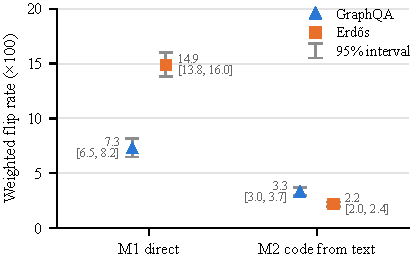
\includegraphics[width=0.48\textwidth]{figures/fig3_weighted_by_mode.pdf}
\caption{Weighted flip rate (mean $D$ over all tuples) of M1 and M2 under relabeling and edge order. M2 is averaged over plain Python and NetworkX. Whiskers are 95\% confidence intervals over the choice of graphs, computed as in Figure~\ref{fig:2}.}
\label{fig:3}
\end{figure}

\begin{figure*}[!htbp]
\centering
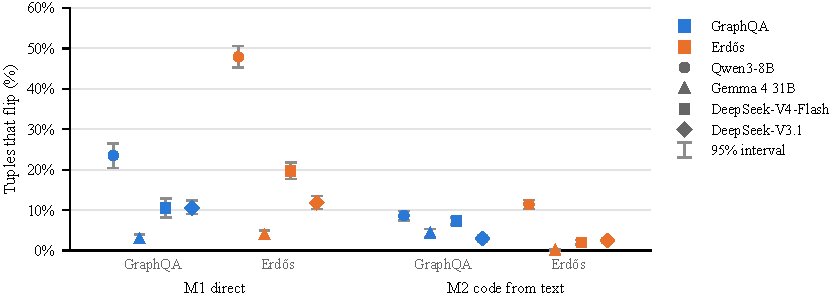
\includegraphics[width=0.8\textwidth]{figures/figB1_flip_by_model.pdf}
\caption{Flip rate of M1 and M2 for each model under relabeling and edge order, as in Figure~\ref{fig:2} but without pooling the models. Color marks the dataset and shape the model. M2 is averaged over plain Python and NetworkX. Whiskers are 95\% confidence intervals over the choice of graphs, computed as in Figure~\ref{fig:2}.}
\label{fig:B1}
\end{figure*}

\begin{figure*}[!htbp]
\centering
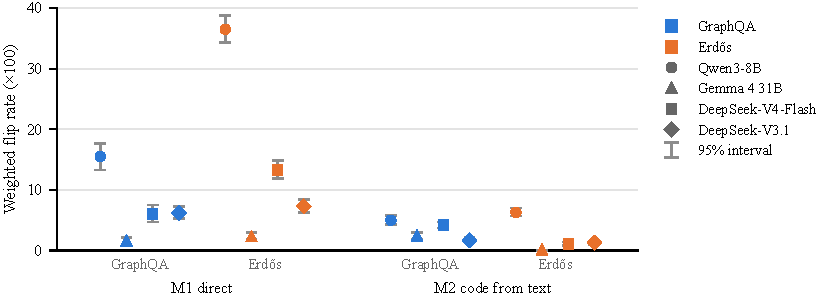
\includegraphics[width=0.8\textwidth]{figures/figB2_weighted_by_model.pdf}
\caption{Weighted flip rate (mean $D$ over all tuples) for each model under relabeling and edge order, as in Figure~\ref{fig:3}. Whiskers as in Figure~\ref{fig:B1}.}
\label{fig:B2}
\end{figure*}

\begin{figure}[!htbp]
\centering
\begin{minipage}[t]{0.48\textwidth}
\centering
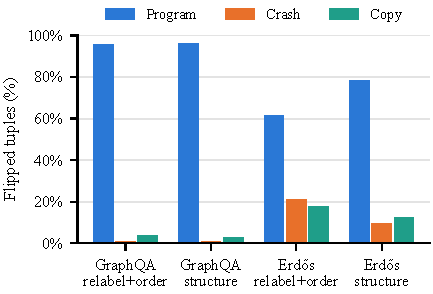
\includegraphics[width=\linewidth]{figures/fig5_where_flips_start.pdf}
\caption{Where plain-Python flips start. The flips of the four models are pooled, so a model with more flips weighs more.}
\label{fig:5}
\end{minipage}\hfill
\begin{minipage}[t]{0.48\textwidth}
\centering
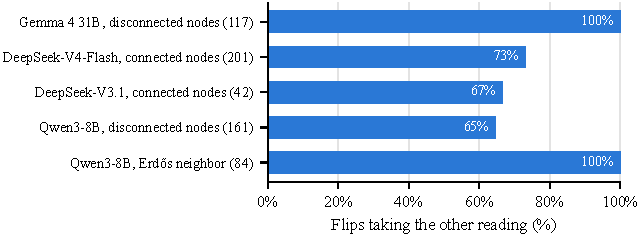
\includegraphics[width=\linewidth]{figures/fig6_other_reading.pdf}
\caption{Share of code flips that contain the answer to the other reading of the question, under relabeling and order, among flips in which every serialization is answered. For Erdős \texttt{neighbor}, whose other reading takes the graph as directed, a flip counts when some answer is a strict subset of the true neighbors. Cells with fewer than 10 flips are left out.}
\label{fig:6}
\end{minipage}
\end{figure}

\begin{table*}[!htbp]
\centering
\begin{minipage}[t]{0.485\textwidth}
\centering
\small\setlength{\tabcolsep}{3.2pt}
\begin{tabular}{@{}lrrrrrr@{}}
\toprule
 & \multicolumn{3}{c}{GraphQA} & \multicolumn{3}{c}{Erd\H{o}s} \\
\cmidrule(lr){2-4} \cmidrule(l){5-7}
Bucket & Dir. & Py & NX & Dir. & Py & NX \\
\midrule
\multicolumn{7}{@{}l}{\emph{Qwen3-8B}} \\
(1) Same, correct & 69.8 & 93.8 & 84.5 & 48.5 & 84.6 & 60.7 \\
(2) Same, wrong & 6.6 & 0.4 & 3.7 & 1.0 & 1.8 & 0.9 \\
(3) Different, all correct & 0.0 & 0.0 & 0.0 & 2.6 & 4.8 & 4.5 \\
(4) Flip, all answered & 22.2 & 5.6 & 9.1 & 42.4 & 7.8 & 1.2 \\
(5) Flip with a crash & 1.2 & 0.1 & 2.3 & 5.5 & 1.0 & 12.8 \\
(6) No answer on all & 0.1 & 0.0 & 0.4 & 0.0 & 0.0 & 20.0 \\
\addlinespace
\multicolumn{7}{@{}l}{\emph{Gemma 4 31B}} \\
(1) Same, correct & 87.5 & 95.3 & 94.6 & 92.2 & 95.5 & 95.6 \\
(2) Same, wrong & 9.5 & 1.0 & 0.5 & 0.1 & 0.0 & 0.0 \\
(3) Different, all correct & 0.0 & 0.0 & 0.0 & 3.7 & 4.4 & 4.2 \\
(4) Flip, all answered & 3.0 & 3.7 & 4.8 & 3.4 & 0.1 & 0.0 \\
(5) Flip with a crash & 0.0 & 0.0 & 0.1 & 0.6 & 0.1 & 0.1 \\
(6) No answer on all & 0.0 & 0.0 & 0.0 & 0.0 & 0.0 & 0.0 \\
\addlinespace
\multicolumn{7}{@{}l}{\emph{DeepSeek-V4-Flash}} \\
(1) Same, correct & 75.7 & 74.9 & 78.6 & 75.3 & 91.5 & 94.8 \\
(2) Same, wrong & 13.8 & 18.0 & 13.9 & 0.7 & 0.6 & 0.4 \\
(3) Different, all correct & 0.0 & 0.0 & 0.0 & 4.3 & 4.4 & 4.2 \\
(4) Flip, all answered & 10.5 & 7.1 & 7.5 & 17.9 & 1.3 & 0.6 \\
(5) Flip with a crash & 0.0 & 0.0 & 0.0 & 1.8 & 2.2 & 0.0 \\
(6) No answer on all & 0.0 & 0.0 & 0.0 & 0.0 & 0.0 & 0.0 \\
\addlinespace
\multicolumn{7}{@{}l}{\emph{DeepSeek-V3.1}} \\
(1) Same, correct & 73.7 & 84.6 & 83.9 & 83.5 & 93.8 & 92.3 \\
(2) Same, wrong & 15.8 & 12.8 & 12.7 & 0.2 & 0.0 & 0.0 \\
(3) Different, all correct & 0.0 & 0.0 & 0.0 & 4.4 & 4.6 & 4.4 \\
(4) Flip, all answered & 10.4 & 2.6 & 0.9 & 6.9 & 1.5 & 2.0 \\
(5) Flip with a crash & 0.1 & 0.0 & 2.4 & 4.9 & 0.1 & 1.3 \\
(6) No answer on all & 0.0 & 0.0 & 0.1 & 0.0 & 0.0 & 0.0 \\
\bottomrule
\end{tabular}
\caption{Tuples by bucket for each model under relabeling and edge order, as in Table~\ref{tab:1} (\% of tuples). Dir. = M1. Py and NX = M2 in plain Python and with NetworkX.}
\label{tab:B1}
\end{minipage}\hfill
\begin{minipage}[t]{0.485\textwidth}
\centering
\small\setlength{\tabcolsep}{3.2pt}
\begin{tabular}{@{}lrrrrrr@{}}
\toprule
 & \multicolumn{3}{c}{GraphQA} & \multicolumn{3}{c}{Erd\H{o}s} \\
\cmidrule(lr){2-4} \cmidrule(l){5-7}
Factor & Dir. & Py & NX & Dir. & Py & NX \\
\midrule
\multicolumn{7}{@{}l}{\emph{Qwen3-8B}} \\
Relabeling & \textbf{24.3} & 7.3 & \textbf{12.7} & \textbf{49.2} & 8.9 & \textbf{14.4} \\
Order & \textbf{22.6} & 4.2 & \textbf{10.0} & \textbf{46.7} & 8.8 & \textbf{13.6} \\
Structure & \textbf{32.0} & \textbf{40.3}$^\dagger$ & \textbf{18.7} & \textbf{49.5} & \textbf{35.1} & \textbf{28.5} \\
Syntax & \textbf{27.4} & 4.9 & \textbf{39.3}$^\dagger$ & \textbf{49.1} & 9.9 & \textbf{34.2} \\
\addlinespace
\multicolumn{7}{@{}l}{\emph{Gemma 4 31B}} \\
Relabeling & 3.3 & 4.1 & 5.6$^\dagger$ & 4.3 & 0.2 & 0.2 \\
Order & 2.8 & 3.2 & 4.2$^\dagger$ & 3.6 & 0.2 & 0.0 \\
Structure & 9.3 & 2.7 & 3.1 & 3.3 & 0.9 & 1.4 \\
Syntax & 6.9 & 3.6 & 4.3 & 2.6 & 0.4 & 0.8 \\
\addlinespace
\multicolumn{7}{@{}l}{\emph{DeepSeek-V4-Flash}} \\
Relabeling & \textbf{11.9} & 7.9 & 7.3 & \textbf{21.9} & 3.4 & 0.6 \\
Order & 9.1 & 6.2 & 7.7 & \textbf{17.4} & 3.6 & 0.6 \\
Structure & \textbf{16.9} & \textbf{17.0} & 7.3 & \textbf{15.8} & \textbf{11.4} & 7.8 \\
Syntax & \textbf{13.3} & 7.6 & 6.7 & \textbf{15.8} & 4.3 & \textbf{29.7}$^\dagger$ \\
\addlinespace
\multicolumn{7}{@{}l}{\emph{DeepSeek-V3.1}} \\
Relabeling & \textbf{11.0} & 3.0 & 3.3 & \textbf{13.0} & 1.8 & 3.4 \\
Order & \textbf{10.0} & 2.2 & 3.3 & \textbf{10.7} & 1.5 & 3.2 \\
Structure & \textbf{18.7} & \textbf{14.0} & 2.9 & 9.4 & 7.4 & 3.1 \\
Syntax & \textbf{12.0} & 3.3 & 4.1 & 8.2 & 0.7 & 1.6 \\
\bottomrule
\end{tabular}
\caption{Flip rate by factor for each model, as in Table~\ref{tab:2} (\% of tuples). Bold: 10\% or more. $^\dagger$: the model's code flips at least 1 point more often than its own direct answers.}
\label{tab:B2}
\end{minipage}
\end{table*}

\FloatBarrier
\section[Setup and Metric Details]{ Setup and Metric Details}\label{app:tuples}

\begin{figure}[!htbp]
\centering
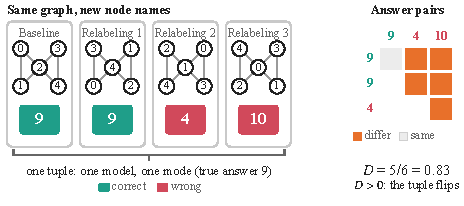
\includegraphics[width=0.6\textwidth]{figures/fig1_tuple.pdf}
\caption{One tuple: Qwen3-8B answering Erdős triangles-0000 directly under four labelings of one graph (drawn schematically). Green answers are correct, red wrong. Five of the six answer pairs differ, so $D = 0.83$.}
\label{fig:1}
\end{figure}

\begin{table*}[!htbp]
\centering
\small
\begin{tabular}{@{}p{0.11\textwidth}p{0.33\textwidth}p{0.22\textwidth}p{0.26\textwidth}@{}}
\toprule
Factor & Answers in a tuple & GraphQA & Erdős \\
\midrule
Relabeling & baseline labeling + 3 random relabelings & 4 (699 tuples), 3 (1) & 4 (1,199), 3 (1) \\
Order & dataset's own order + 3 reorderings & 4 (587), 3 (63), 2 (39) & 4 (1,133), 3 (58), 2 (9) \\
Structure & baseline + adjacency list + each edge in both directions & 3 (700) & 3 (1,123), 2 (77) \\
Syntax & baseline + plain text, JSON, NetworkX code & 4 (700) & 3, no plain text (1,200) \\
\bottomrule
\end{tabular}
\caption{Answers per tuple, with the number of tuples of each size per model and mode. A serialization identical to its baseline is dropped, which shortens some tuples: 11 GraphQA instances have no order tuple, one random relabeling per dataset came out as the identity, and the 77 directed Erdős graphs have no both-directions serialization.}
\label{tab:D1}
\end{table*}

\FloatBarrier
\section{M3 Without the Stated Graph Type}\label{app:m3first}

\begin{table}[!htbp]
\centering
\small\setlength{\tabcolsep}{4pt}
\begin{tabular}{@{}lrrrrr@{}}
\toprule
 & M1 & \multicolumn{2}{c}{M2} & \multicolumn{2}{c}{M3} \\
\cmidrule(lr){3-4} \cmidrule(l){5-6}
 &  & Py & NX & Py & NX \\
\midrule
\multicolumn{6}{@{}l}{\emph{Accuracy, all serializations}} \\
GraphQA & 84.4 & 88.3 & 88.8 & \textbf{92.9} & 87.0 \\
Erdős & 87.0 & \textbf{96.9} & 91.1 & 91.2 & 84.2 \\
\addlinespace
\multicolumn{6}{@{}l}{\emph{Robust accuracy, relabeling and order}} \\
GraphQA & 76.7 & 87.2 & 85.4 & \textbf{92.2} & 86.8 \\
Erdős & 78.6 & \textbf{95.9} & 90.2 & 91.0 & 84.1 \\
\bottomrule
\end{tabular}
\caption{Table~\ref{tab:3} with the first M3 run on Erdős, before the graph type was stated in its prompt. M1, M2 and all of GraphQA are unchanged. Bold: highest in the row.}
\label{tab:E1}
\end{table}

\end{document}
